%package list
\documentclass{article}
\usepackage[top=3cm, bottom=3cm, outer=3cm, inner=3cm]{geometry}
\usepackage{graphicx}
\usepackage{url}
\usepackage{multirow}
%\usepackage{cite}
\usepackage{hyperref}
\usepackage{array}
\usepackage{multicol}
\newcolumntype{x}[1]{>{\centering\arraybackslash\hspace{0pt}}p{#1}}
\usepackage{natbib}
\usepackage{pdfpages}
\usepackage{multirow}
\usepackage{float}
\usepackage[normalem]{ulem}
\useunder{\uline}{\ul}{}




%%%%%%%%%%%%%%%%%%%%%%%%%%%%%%%%%%%%%%%%%%%%%%%%%%%%%%%%%%%%%%%%%%%%%%%%%%%%
%%%%%%%%%%%%%%%%%%%%%%%%%%%%%%%%%%%%%%%%%%%%%%%%%%%%%%%%%%%%%%%%%%%%%%%%%%%%
\newcommand{\csemail}{vmachacaa@unsa.edu.pe}
\newcommand{\csdocente}{Vicente Machaca Arceda}
\newcommand{\cscurso}{Algoritmos y Estructura de Datos}
\newcommand{\csuniversidad}{Universidad Nacional de San Agustín}
\newcommand{\csescuela}{Maestría en Ciencia de la Computación}
\newcommand{\cspracnr}{01}
\newcommand{\cstema}{--}
%%%%%%%%%%%%%%%%%%%%%%%%%%%%%%%%%%%%%%%%%%%%%%%%%%%%%%%%%%%%%%%%%%%%%%%%%%%%
%%%%%%%%%%%%%%%%%%%%%%%%%%%%%%%%%%%%%%%%%%%%%%%%%%%%%%%%%%%%%%%%%%%%%%%%%%%%


\usepackage[english,spanish]{babel}
\usepackage[utf8]{inputenc}
\AtBeginDocument{\selectlanguage{spanish}}
\renewcommand{\figurename}{Figura}
\renewcommand{\refname}{Referencias}
\renewcommand{\tablename}{Tabla} %esto no funciona cuando se usa babel
\AtBeginDocument{%
	\renewcommand\tablename{Tabla}
}

\usepackage{fancyhdr}
\pagestyle{fancy}
\fancyhf{}
\setlength{\headheight}{30pt}
\renewcommand{\headrulewidth}{1pt}
\renewcommand{\footrulewidth}{1pt}
\fancyhead[L]{\raisebox{-0.2\height}{
\includegraphics[width=3cm]{Img/logo_unsa.jpg}}}
\fancyhead[C]{}
\fancyhead[R]{\fontsize{7}{7}\selectfont	\csuniversidad \\ \csescuela \\ \textbf{\cscurso} }
\fancyfoot[L]{MSc. Vicente Machaca}
\fancyfoot[C]{\cscurso}
\fancyfoot[R]{Página \thepage}







\begin{document}
	
	\vspace*{10px}
	
	\begin{center}	
		\fontsize{17}{17} \textbf{ Práctica \cspracnr}
	\end{center}
	%\centerline{\textbf{\underline{\Large Título: Informe de revisión del estado del arte}}}
	%\vspace*{0.5cm}
	

	\begin{table}[h]
		\begin{tabular}{|x{4.7cm}|x{4.8cm}|x{4.8cm}|}
			\hline 
			\textbf{DOCENTE} & \textbf{CARRERA}  & \textbf{CURSO}   \\
			\hline 
			\csdocente & \csescuela & \cscurso    \\
			\hline 
		\end{tabular}
	\end{table}	
	
	
	\begin{table}[h]
		\begin{tabular}{|x{4.7cm}|x{4.8cm}|x{4.8cm}|}
			\hline 
			\textbf{PRÁCTICA} & \textbf{TEMA}  & \textbf{DURACIÓN}   \\
			\hline 
			\cspracnr & Algoritmos de ordenamiento  & 3 horas   \\
			\hline 
		\end{tabular}
	\end{table}
	
	
	\section{Datos de los estudiantes}
	Grupo: N° 8
	\begin{itemize}
		\item Integrantes: 
		\begin{itemize}
			\item Esai Josue Huaman Meza
			\item Alan Jerry Reyes Robles
			\item Jorge Luis Zegarra Guardamino
			\item Nestor Giraldo Calcinas Huaranga
		\end{itemize}		
	\end{itemize}
	
	
	
	
	
	
	\section{Introducción}
	
	Para esta Práctica, se implemetará las estructuras de datos AVL y B-Tree. Para cada estructura se deben de implemetar lo métodos Insert, Delete, Minimum, Maximum y Search. Para implemetar estas estructuras se usará el lenguaje de programación Python.

    Una ves obtenido las estructuras, se mostrarán los resultados de manera gráfica, el cual será XXXXXXXXXXXX
	
	
	\section{Estructuras de Datos}\label{sec:ejercicios}
	\begin{enumerate}
		\item \textbf{Estructura de datos AVL}
		
			Una estrucutra de Datos AVL, también llamado árbol de datos AVL es un tipo especial de arbol binario ideado por los matemáticos soviéticos Adelson-Velskii y Landis. Fue el primer árbol de búsqueda binario auto-balanceable que se ideó.

La Esturctura AVL se describe de la siguiente manera: 

\begin{itemize}
   \item Los árboles AVL están siempre equilibrados de tal modo que para todos los nodos, la altura de la rama izquierda no difiere en más de una unidad de la altura de la rama derecha o viceversa.
   \item Gracias al equilibrio (o balanceo), la complejidad de una búsqueda en uno de estos árboles se mantiene siempre en orden de complejidad O(log n).
   \item El factor de equilibrio puede ser almacenado directamente en cada nodo o ser computado a partir de las alturas de los subárboles.
   \item Para conseguir esta propiedad de equilibrio, la inserción y el borrado de los nodos se ha de realizar de una forma especial.
   \item Si al realizar una operación de inserción o borrado se rompe la condición de equilibrio, hay que realizar una serie de rotaciones de los nodos.
   \item Los árboles AVL más profundos son los árboles de Fibonacci.
\end{itemize}	

 Factor de Esquilibrio en la Estructura AVL:

 \begin{itemize}
   \item El factor de equilibrio es la diferencia entre las alturas del árbol derecho y el izquierdo:
   
   FE = altura subárbol derecho - altura subárbol izquierdo
   
   Por definición, para un árbol AVL, este valor debe ser -1, 0 o 1.
   \item Si el factor de equilibrio de un nodo es:
   
   0: El nodo está equilibrado y sus subárboles tienen exactamente la misma altura.
   
   1: El nodo está equilibrado y su subárbol derecho es un nivel más alto.
   
   -1: El nodo está equilibrado y su subárbol izquierdo es un nivel más alto.
   \item Si el factor de equilibrio $\ |Fe|>=2 $ es necesario reequilibrar.
\end{itemize}

Para poder reequilibrar en la Estructura AVL, es necesario realizar operaciones de rotación, las cuales son:

 \begin{itemize}
   \item Rotación simple a la derecha:

\begin{figure}[H]
\centering
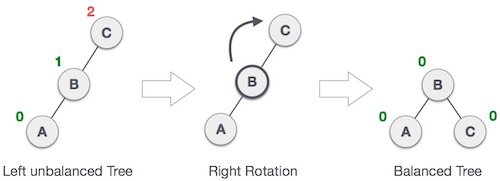
\includegraphics[width=0.7\textwidth]{Img/avl_right_rotation.jpg}
\caption{Rotación Simple Derecha AVL}
\end{figure}
   
   \item Rotación simple a la izquierda:

\begin{figure}[H]
\centering
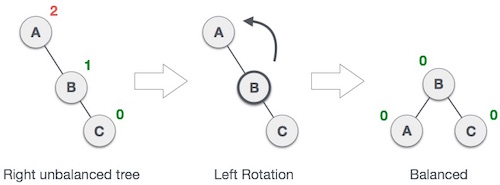
\includegraphics[width=0.7\textwidth]{Img/avl_left_rotation.jpg}
\caption{Rotación Simple Izquierda AVL}
\end{figure}
   
   \item Rotación compleja a la izquierda - derecha y viceversa:

\begin{figure}[H]
\centering
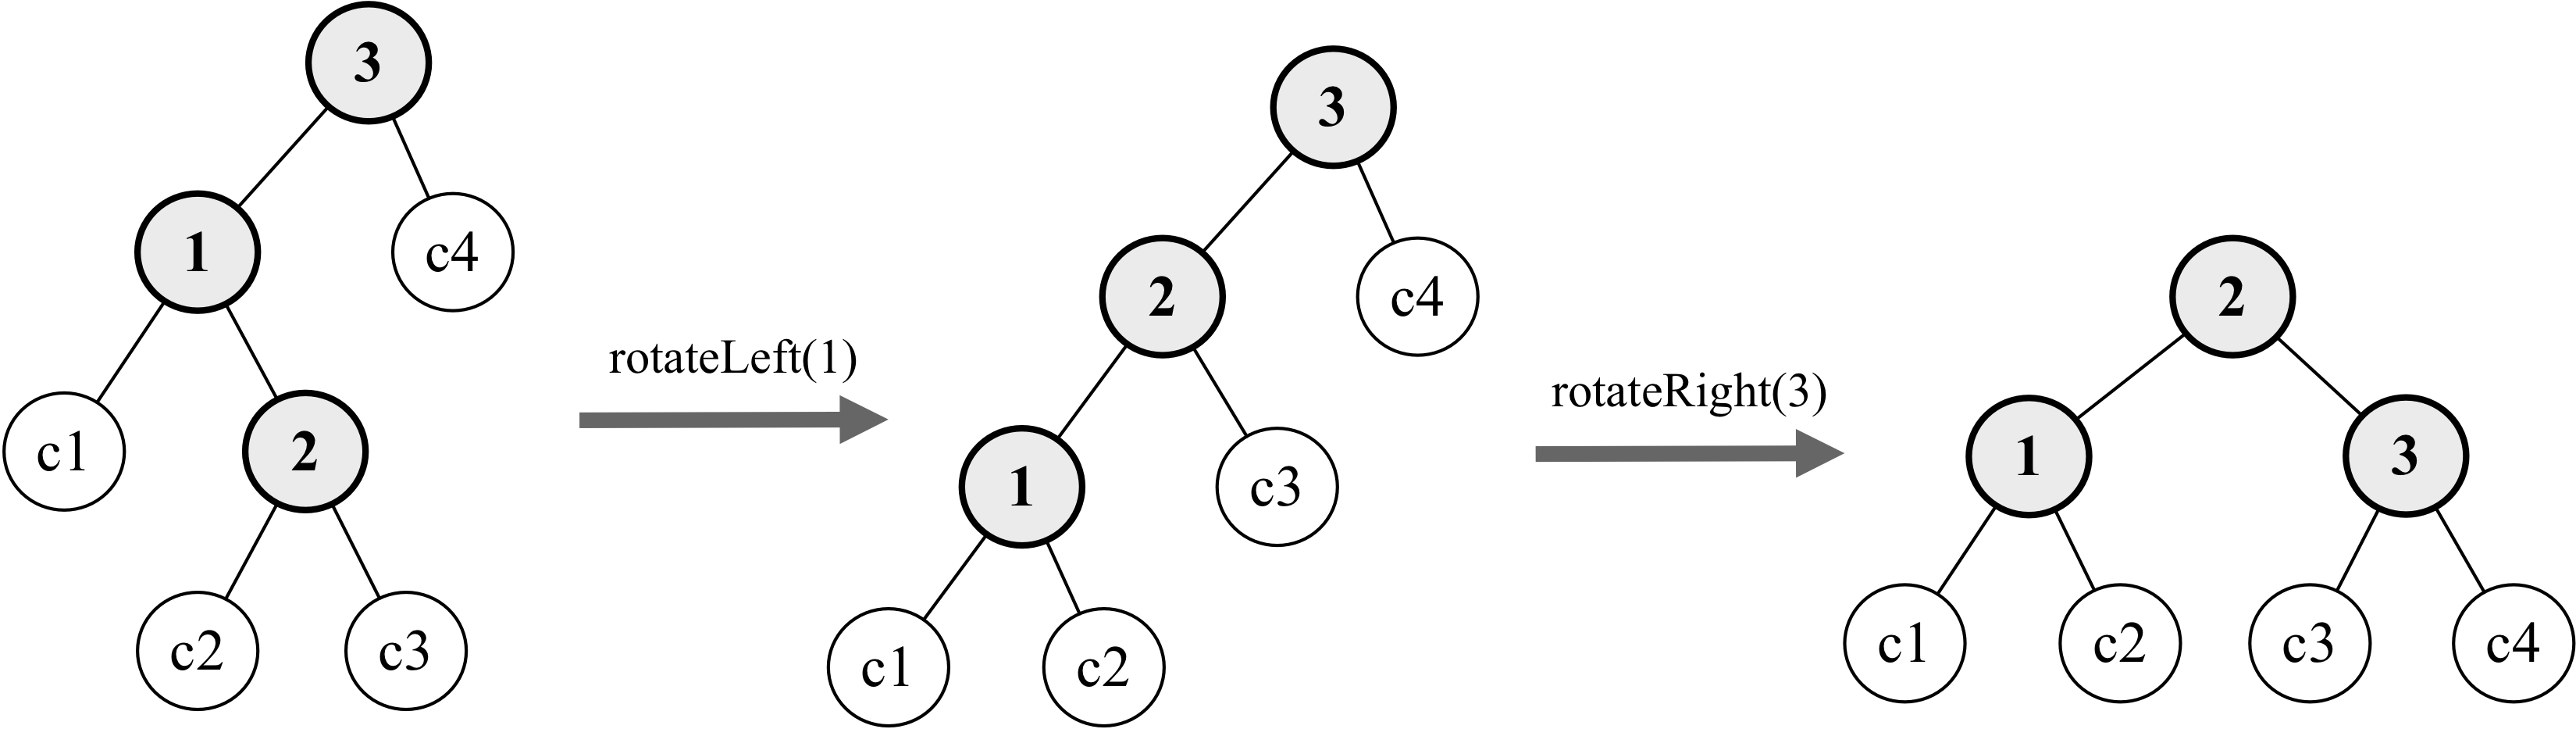
\includegraphics[width=0.9\textwidth]{Img/Rotation_Complex_AVL.png}
\caption{Rotación Compleja AVL}
\end{figure}

\end{itemize}
		

\item \textbf{AEstructura de datos B-Tree}

Son estructuras que se encuentran comúnmente en la implementación de base de datos y sistemas de archivos. Al igual que los árboles binarios de búsqueda, son árboles balanceados de búsqueda, pero cada nodo puede poseer más de dos hijos. Los árboles B-Tree mantienen los datos ordenados y las inserciones y eliminaciones se realizan en tiempo logarítmico amortizado.

La Esturctura B-Tree se describe de la siguiente manera: 

\begin{itemize}
   \item Cada elemento de un nodo interno actúa como un valor separador, que lo divide en subárboles. Si un nodo interno tiene tres nodos hijo, debe tener dos valores separadores o elementos a1 y a2. Todos los valores del subárbol izquierdo deben ser menores a a1, todos los valores del subárbol del centro deben estar entre a1 y a2, y todos los valores del subárbol derecho deben ser mayores a a2.
   \item Los nodos internos del B-Tree, es decir los nodos que no son hoja, usualmente se representan como un conjunto ordenado de elementos y punteros a los hijos.
   \item Los nodos hoja tienen la misma restricción sobre el número de elementos, pero no tienen hijos, y por tanto carecen de punteros.
   \item El nodo raíz tiene límite superior de número de hijos, pero no tiene límite inferior.
   \item Los Los árboles B-Tree guardan valores en cada nodo, y pueden utilizar la misma estructura para todos los nodos.
\end{itemize}

\begin{figure}[H]
\centering
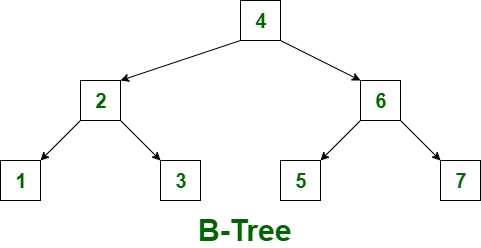
\includegraphics[width=0.7\textwidth]{Img/B-Tree.png}
\caption{Estructura B-Tree Simple}
\end{figure}

Para poder reequilibrar en B-Tree, si al eliminar un elemento de un nodo hoja, el nodo se ha quedado con menos elementos que el mínimo permitido, algunos elementos se deben redistribuir. En algunos casos el cambio lleva a la deficiencia al nodo padre, y la redistribución se debe aplicar iterativamente hacia arriba del árbol, quizá incluso hasta a la raíz. Dado que la cota mínima en el número de elementos no se aplica a la raíz. 
		 
\end{enumerate}


\section{Implementación}

  Se desarrollan las estructuras AVL y B-Tree implementando los métodos Insert, Delete, Minimum, Maximum y Search, los cuales se pueden encontrar en el siguiente repositorio Github \href{https://github.com/josuemzx/Algoritmos_de_ordenamiento-/blob/main/QuickSort.ipynb}{Estructuras de Datos}, y se obtiene los siguientes gráficos.


\section{Resultados}


    \begin{enumerate}
    
        \item Estructura AVL
        \item Estructura B-Tree
        
    \end{enumerate}

\section{Conclusiones}

\begin{itemize}
            \item 1
\end{itemize}
\begin{itemize}
            \item 2
\end{itemize}

\begin{itemize}
            \item 3
\end{itemize}    
\begin{itemize}
            \item 4
\end{itemize}
\begin{itemize}
            \item 5
\end{itemize}	
	%\clearpage
	%\bibliographystyle{apalike}
	%\bibliographystyle{IEEEtranN}
	%\bibliography{bibliography}
		
	
\end{document}
